\documentclass{beamer}

\usepackage{xcolor}
\usepackage{hyperref}

\hypersetup{
    colorlinks=true,
    linkcolor=blue,
    urlcolor=blue
}
% -------------------------------------------------
% Theme and Styling
% -------------------------------------------------

\usetheme{Madrid}



% Remove navigation symbols and footer
\setbeamertemplate{navigation symbols}{}
\setbeamertemplate{footline}{}


% --- Custom Header (Makes Title Clearly Visible) ---
\setbeamertemplate{frametitle}{
    \vspace{0.2em}
    \begin{beamercolorbox}[wd=\paperwidth,ht=3ex,dp=1.2ex,
        leftskip=1em,rightskip=1em]{frametitle}
        \usebeamerfont{frametitle}\insertframetitle
    \end{beamercolorbox}
}

% Old Dominion University-inspired colors
\definecolor{ODUNavy}{RGB}{0,38,84}
\definecolor{ODUSilver}{RGB}{167,169,172}

\setbeamercolor{title}{fg=ODUNavy}
\setbeamercolor{frametitle}{fg=white,bg=ODUNavy}
\setbeamercolor{structure}{fg=ODUNavy}
\setbeamercolor{normal text}{fg=black,bg=white}

\usepackage{graphicx}
\usepackage{hyperref}

% -------------------------------------------------
% Title Information
% -------------------------------------------------

\title{Statistical Estimation for BGG Ratings}

\author{Liam Whitenack \\
DASC 605 \\
Professor Trent Buskirk \\
Old Dominion University}

\date{\today}

% -------------------------------------------------
\begin{document}
% -------------------------------------------------

% Title Slide
\begin{frame}[plain]
\centering

\vspace{1.5cm}

{\Huge\bfseries\textcolor{ODUNavy}{Statistical Estimation for BGG Ratings}}

\vspace{1cm}

{\large Liam Whitenack}

DASC 605

Professor Trent Buskirk

Old Dominion University

\vspace{1cm}

{\small \today}

\end{frame}

% -------------------------------------------------
% Data Slide
% -------------------------------------------------

\begin{frame}{Data}
\small
\begin{itemize}
\item Collected in August 2025 and March 2026
\item Source: \href{https://boardgamegeek.com/wiki/page/BGG_XML_API2}{BoardGameGeek XML API}
\item Processing code: \href{https://github.com/LiamWhitenack/board-game-geek.git}{GitHub Repository}
\item A much more minimal copy can be downloaded by pressing this \href{https://boardgamegeek.com/data_dumps/bg_ranks}{link}
\end{itemize}
\end{frame}

\begin{frame}[fragile]{Fetching Game Data from BoardGameGeek}

\begin{verbatim}
def fetch_things(
    ids: Iterable[int], max_retries: int, retries: int
) -> list[dict]:
    url = f"`url`/thing?id={','.join(map(str, ids))}&stats=1"
    retries = 0
    while retries < max_retries:
        response = requests.get(url)
        if response.status_code == 200:
            return parse(response.text)["items"]["item"]
        else:
            time.sleep(5)
    raise Exception()
\end{verbatim}

\end{frame}

% -------------------------------------------------
% Full-Screen Graph Slides
% -------------------------------------------------

\begin{frame}{Distribution of Ratings}
\centering
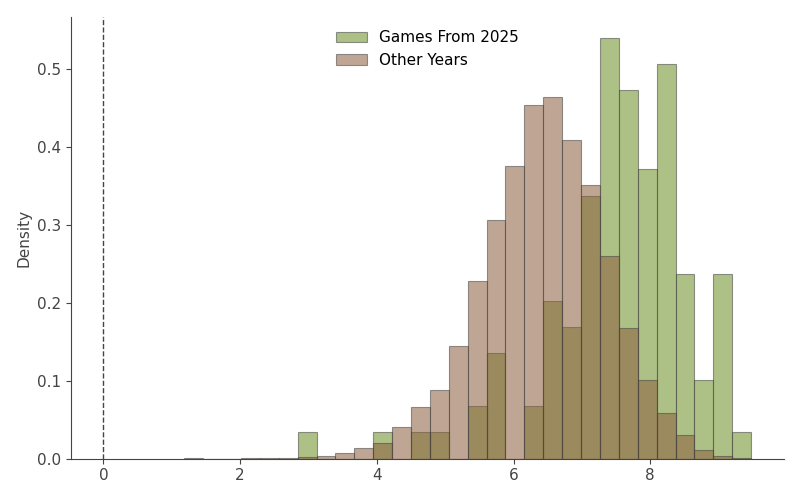
\includegraphics[
width=\paperwidth,
height=\paperheight,
keepaspectratio
]{plots/2025-Ratings-Histogram.png}
\end{frame}

\begin{frame}{Games Published Per Year}
\centering
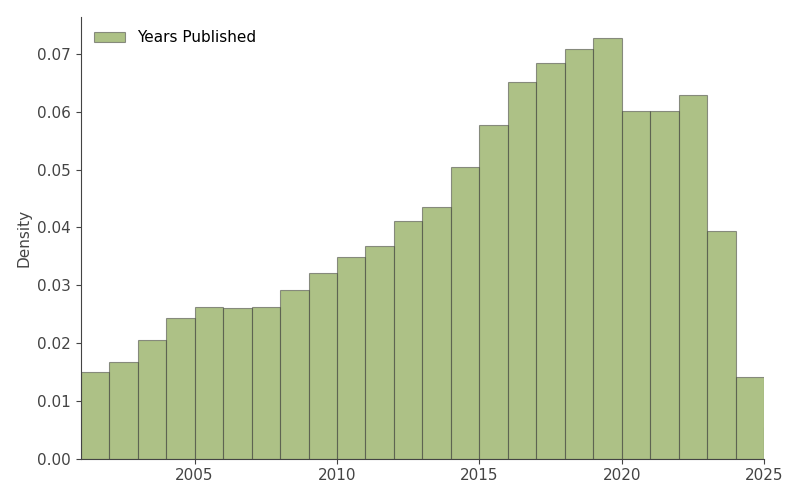
\includegraphics[
width=\paperwidth,
height=\paperheight,
keepaspectratio
]{plots/Board-Games-Published-Per-Year-(Since-2000).png}
\end{frame}

\begin{frame}{Mean Rating by Year}
\centering
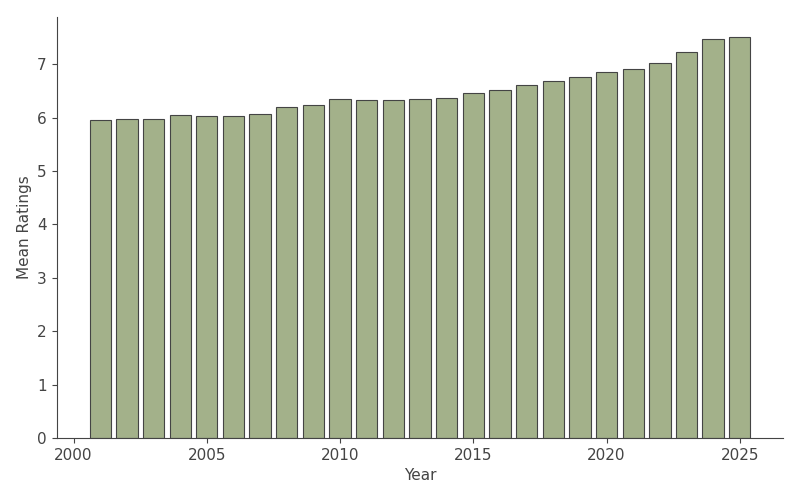
\includegraphics[
width=\paperwidth,
height=\paperheight,
keepaspectratio
]{plots/Mean-Rating-By-Year-(Since-2000).png}
\end{frame}

\begin{frame}{Confidence Interval for Mean Rating}

\textbf{Goal:} Estimate a confidence interval for the true mean rating of a game.

\begin{itemize}
\item Uses the \textbf{t-distribution} because the population standard deviation is unknown.
\item Standard error is computed from the sample ratings.
\item Degrees of freedom: $df = n - 1$
\end{itemize}

\medskip

\textbf{Implementation}

\begin{verbatim}
def confidence_interval_t(self, confidence: float = 0.95) -> tuple[float, float]:
    self._validate_rating_data()

    se = self._standard_error()
    df = self.usersrated - 1
    t_crit = stats.t.ppf((1 + confidence) / 2, df)

    margin = t_crit * se
    return (self.average - margin, self.average + margin)
\end{verbatim}

\end{frame}

\begin{frame}{Top 25 Games}
\centering
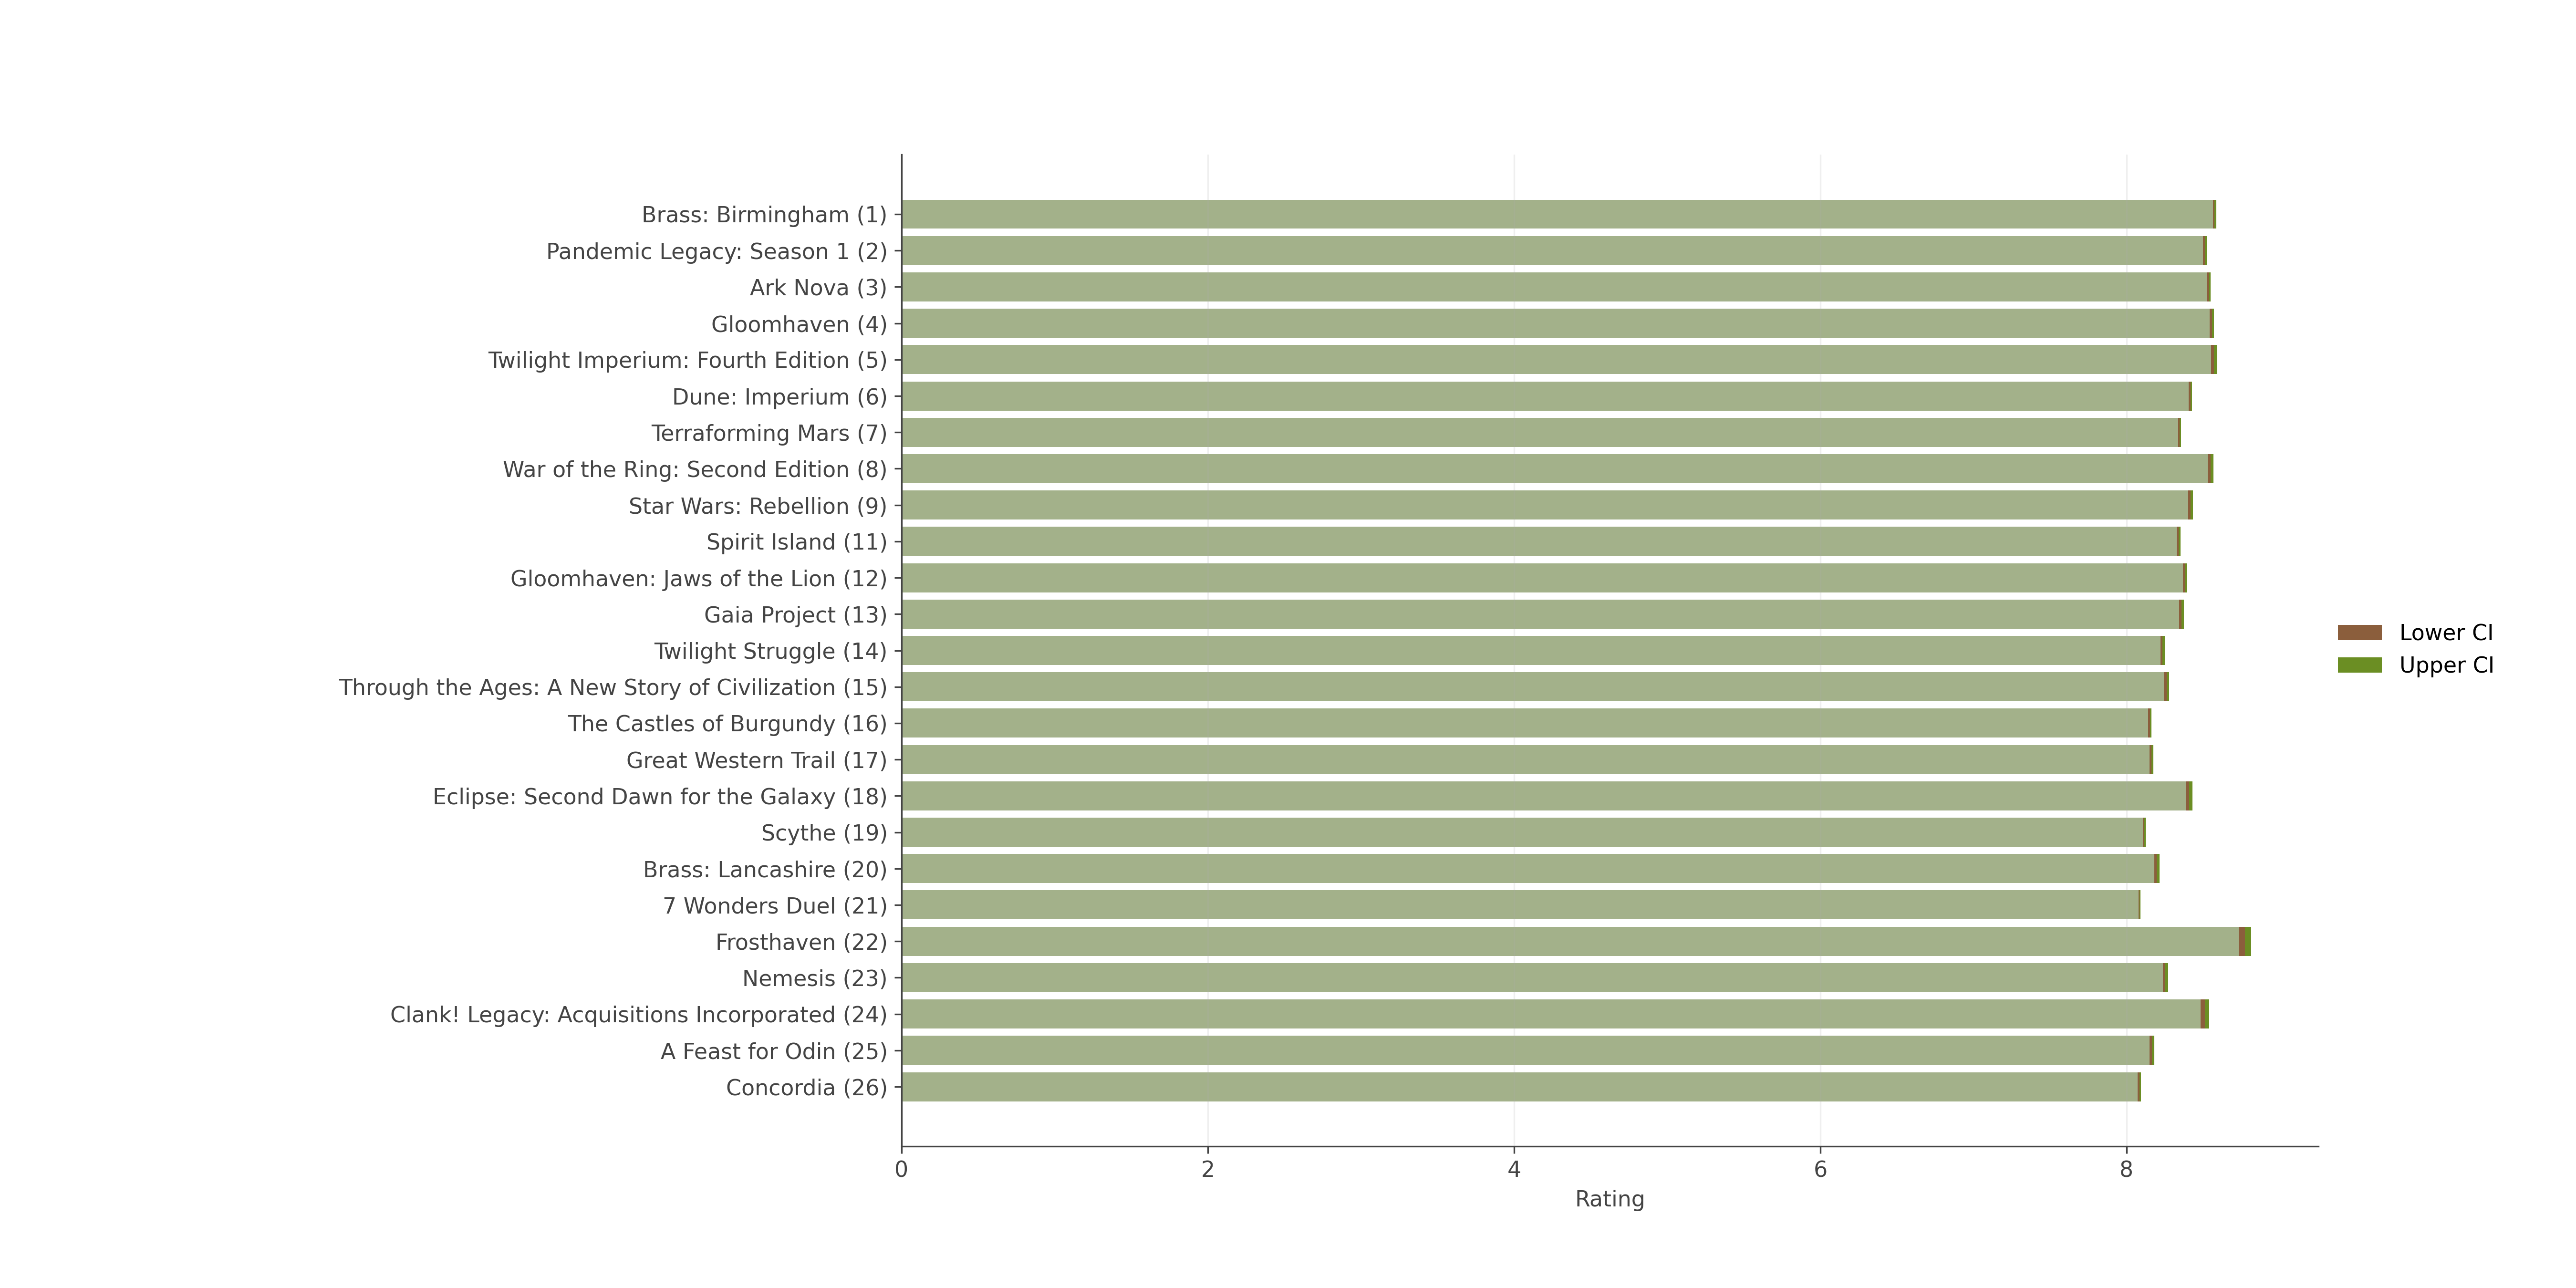
\includegraphics[
width=\linewidth,
height=0.9\textheight,
keepaspectratio
]{plots/Top-25-Games-Ratings-Confidence-Interval.png}
\end{frame}

\begin{frame}{Top 25 Games vs. 2025 Releases}
\centering
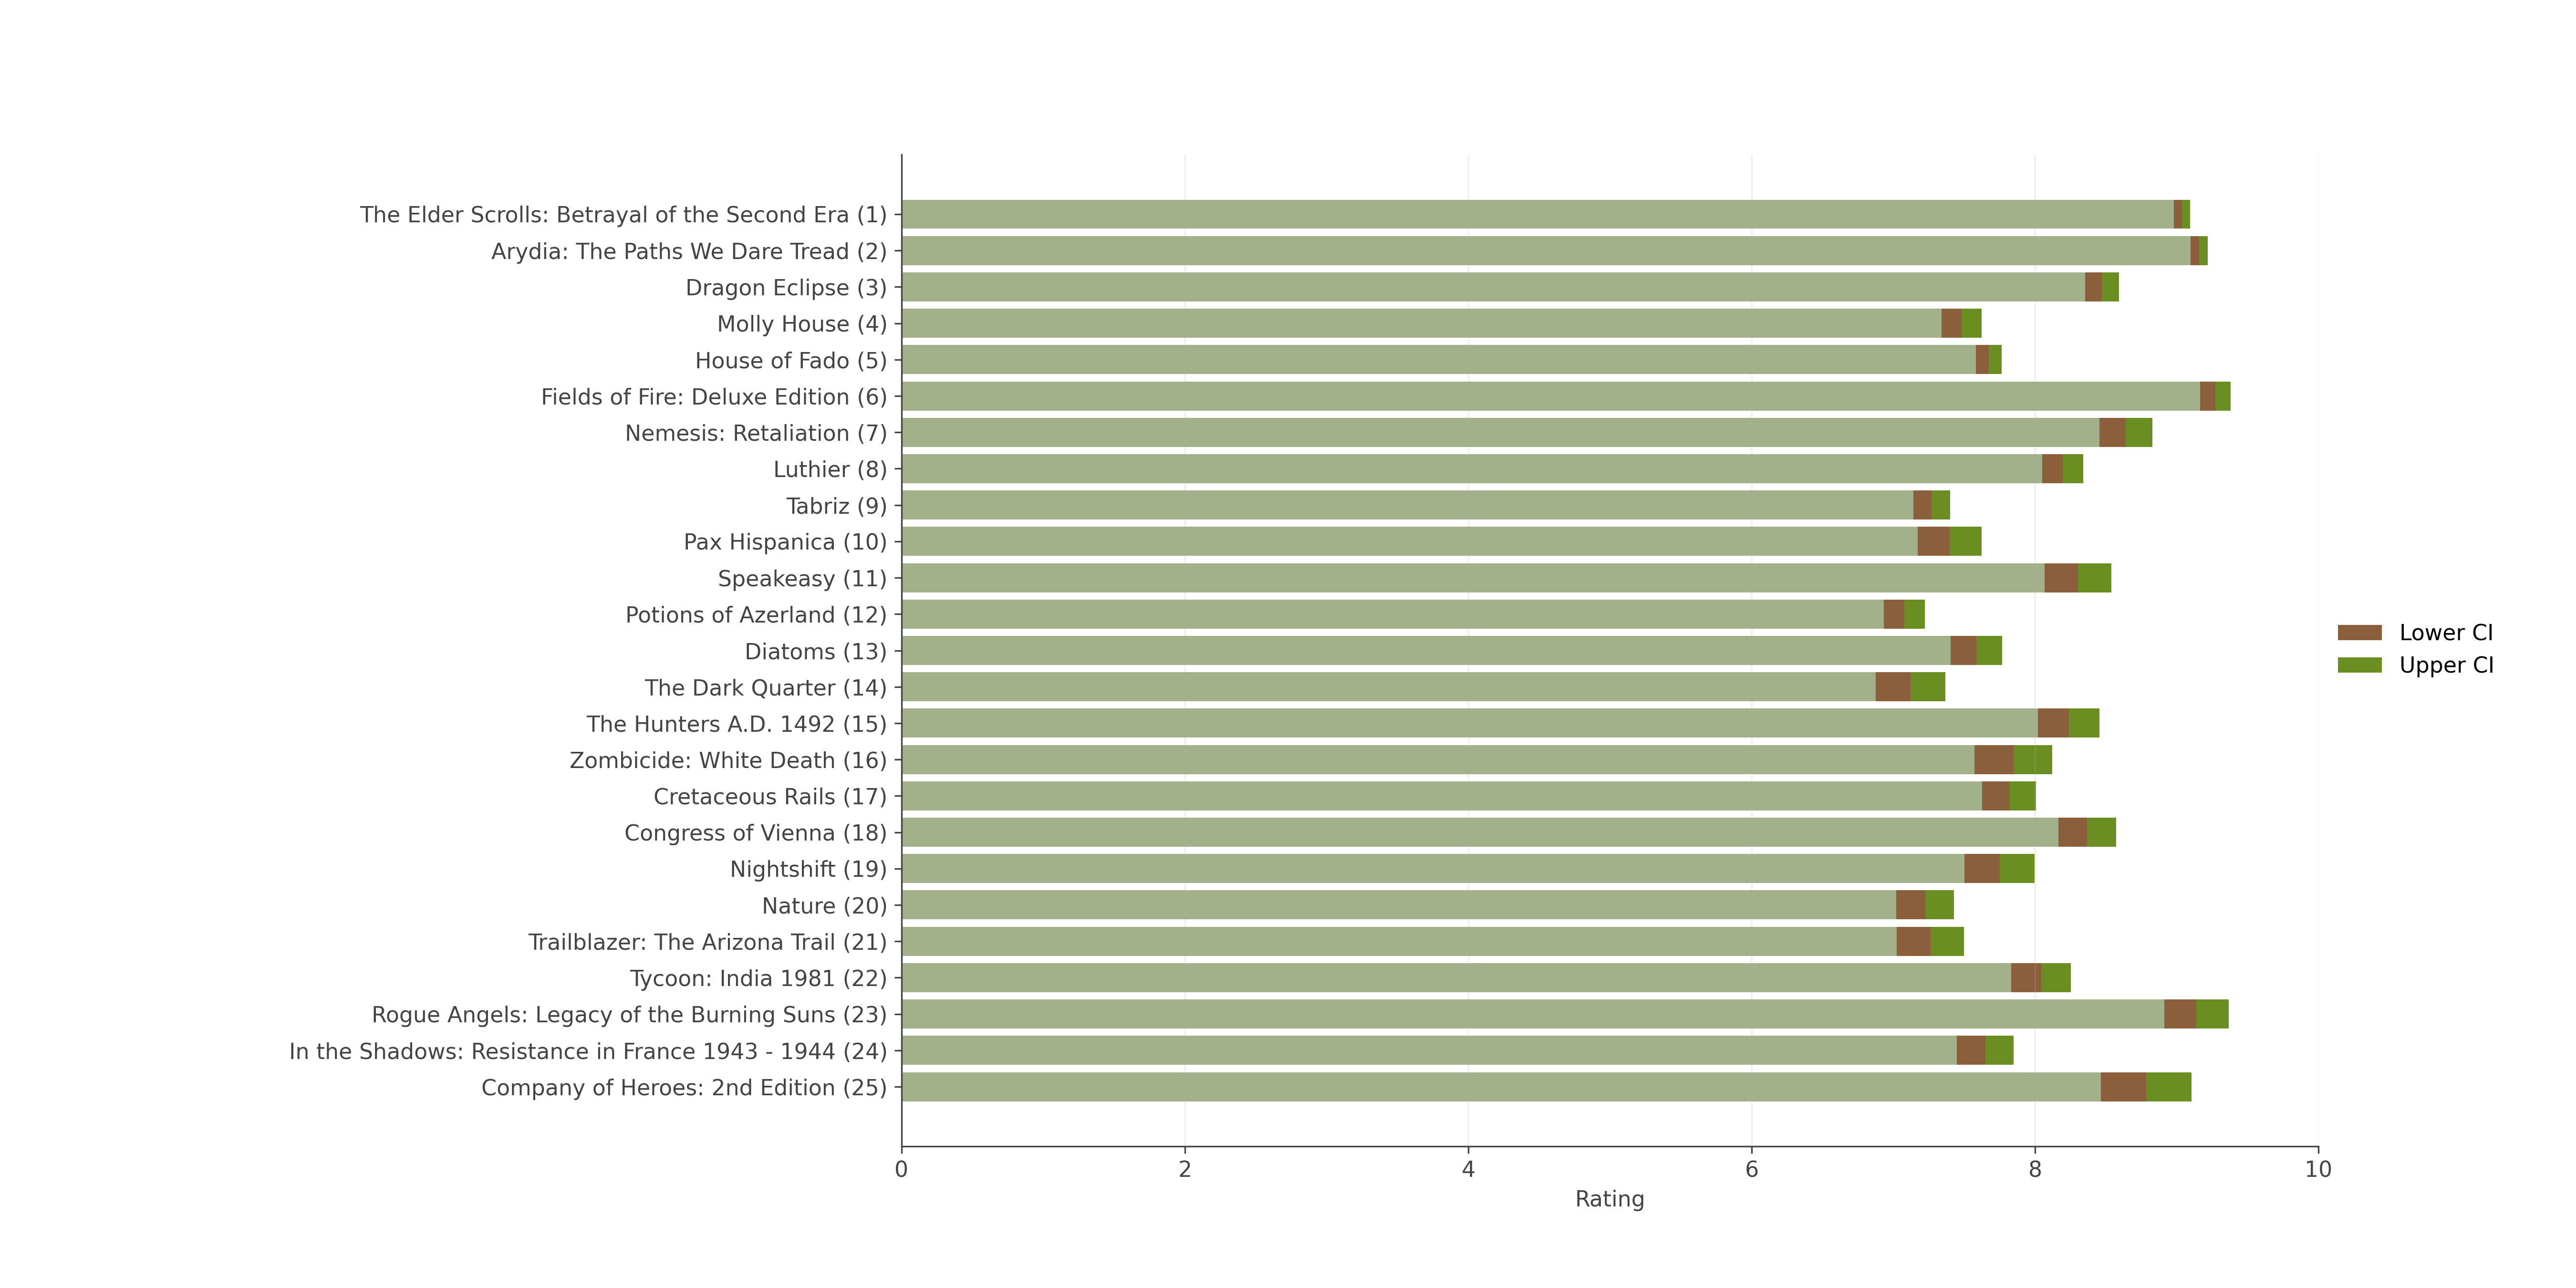
\includegraphics[
width=\linewidth,
height=0.9\textheight,
keepaspectratio
]{plots/Top-25-Games-of-2025-Ratings-Confidence-Interval.png}
\end{frame}

\begin{frame}{Updated 2025 Comparison}
\centering
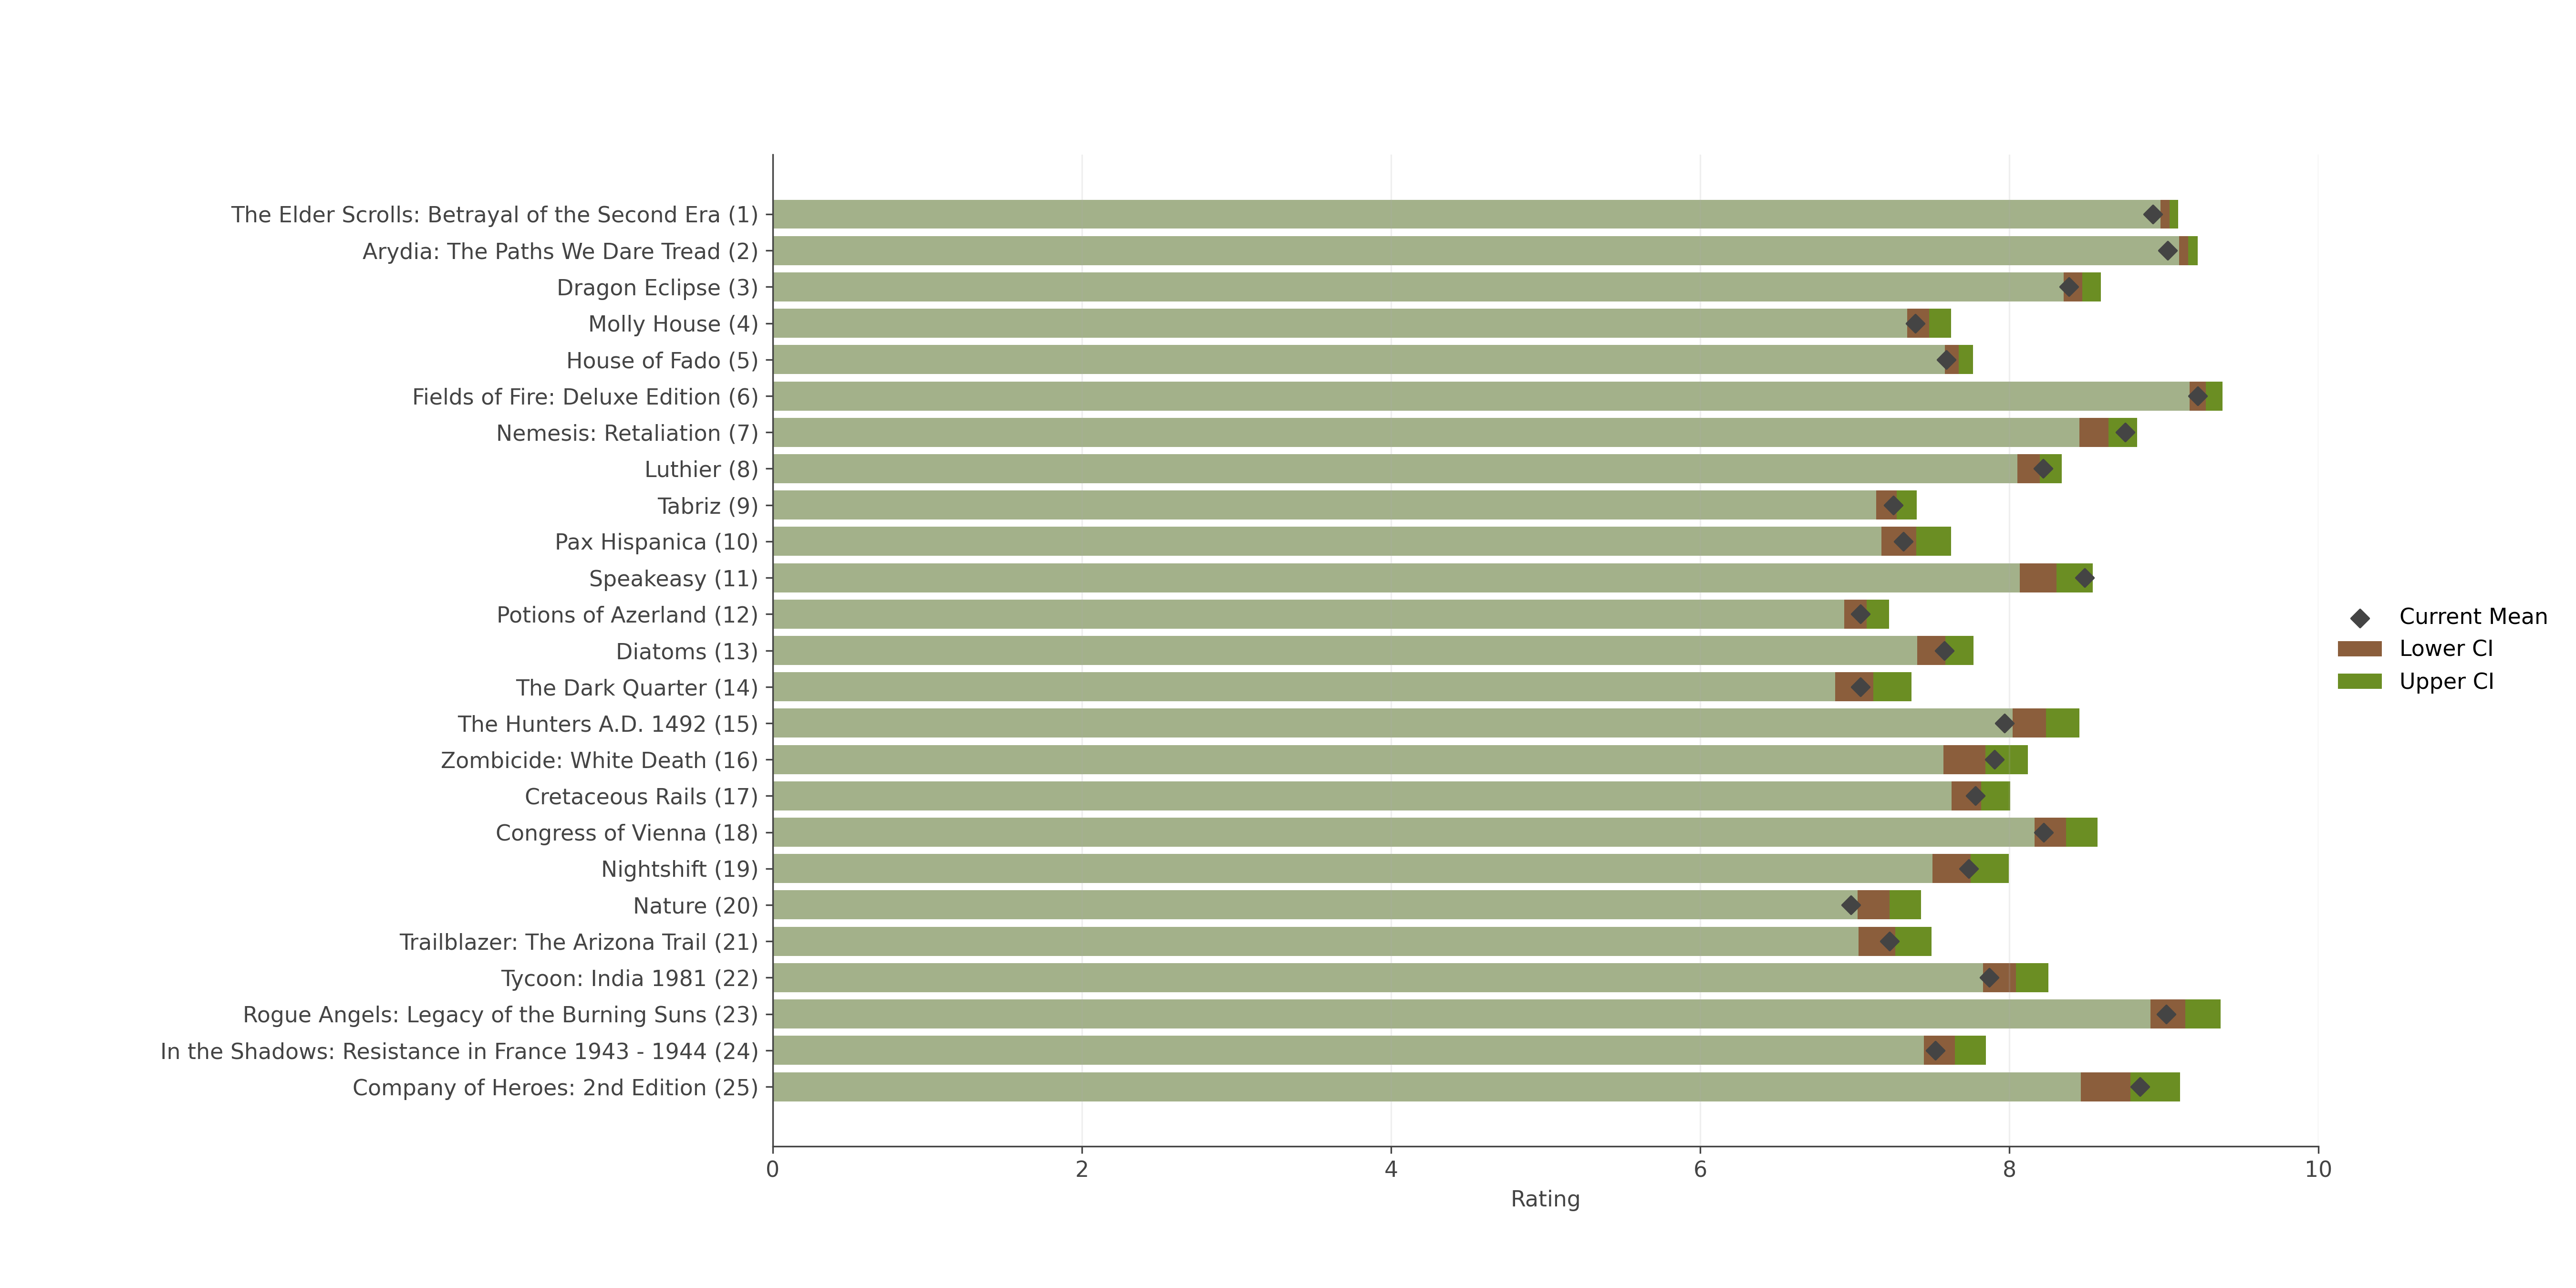
\includegraphics[
width=\linewidth,
height=0.9\textheight,
keepaspectratio
]{plots/Top-25-Games-of-2025-Ratings-Confidence-Interval-Updated.png}
\end{frame}

\end{document}